%%%%%%%%%%%%%%%%%%%%%%%%%%%%
% Master's Thesis          %	    										
% Fabian Burth, 2022-08-01 %
%%%%%%%%%%%%%%%%%%%%%%%%%%%%

\npchapter{Foundations}
\section{Terminology}
This section explains several abbreviations and standards which are frequently mentioned alongside the topics \textit{Vulnerability Management} and \textit{Open Source Licensing} and are thus essential for the further understanding.\\

\subsection{Software Identification}
Uniquely identify a piece of software is a frequent concern when managing applications on enterprise scale. Thus, a standardized naming convention would be required. Unfortunately, pretty much every packet manager and tool uses its own convention.\\

\noindent
\textbf{Package URL (purl)}\\
\noindent
\textit{Package URL}, or purl for short, is one of the most widely adopted attempts to standardize those existing approaches. As described in the projects GitHub Repository, it therefore specifies an URL string, a purl, which should be able "to identify and locate a software package in a mostly universal and uniform way across programming languages, package managers, packaging conventions, tools, APIs and databases" \cite{purl}. This Package URL consists of seven components \cite{purl}:\\

\begin{lstlisting}[caption=Package URL, captionpos=b, label=lst:Purl]
scheme:type/namespace/name@version?qualifiers#subpath
\end{lstlisting}

\begin{lstlisting}[caption=Package URL Examples, captionpos=b, label=lst:Purl]
pkg:docker/cassandra@sha256:244fd47e07d1004f0aed9c
pkg:github/package-url/purl-spec@244fd47e07d1004f0aed9c
pkg:deb/debian/curl@7.50.3-1?arch=i386&distro=jessie
pkg:npm/foobar@12.3.1
\end{lstlisting}

Each component is separated by a different specific character to allow for unambiguous parsing. The \lstinline|scheme| (Required) is the constant value "pkg" which may be officially registered as an URL scheme in the future. \lstinline|type| (Required) refers to a package protocol such as maven or npm. \lstinline|namespace| (Optional) may be some type-specific prefix such as a Maven groupid, a Docker image owner or a Github user or organization. The \lstinline|name| (Required) and \lstinline|version| (Optional) are the name and version of the software. \lstinline|qualifiers| (Optional) is also type-specific and may be used to provide extra qualifying data such as an OS, architecture or a distribution. With the \lstinline|subpath| (Optional) one may specify a subpath within a package, relative to the package root \cite{purl}.\\

Another convention to uniquely identify packages is the \textit{Common Package Enumeration (CPE)} format which is primarily used in the context of vulnerability management ecosystem. Therefore, the standard will be discussed in the following section.

\subsection{Open Source Software and Licensing}
\textit{Open Source Software} is widely used in modern software development. As to what Open Source Software actually is, the \textit{Open Source Initiative} defined a set of rules, the \textit{Open Source Definition} specifying distribution terms that the license of a software must comply with. Without going into detail and examining all of these terms, this definition generally ensures that such software "can be freely accessed, used, changed, and shared (in modified or unmodified form) by anyone" \cite{OSI}.\par
This description on its own may give the impression that there is no need to keep track of what \textit{OSS Licenses} are used within an enterprise application. But there are still some limitation that \textit{OSS Licenses} can put to the usage, especially the distribution of the software. Specifically, the so called \textit{copyleft} principle and corresponding licenses might pose a challenge to some companies. While OSS generally may be used for commercial purposes, this principle dictates that if a company or individual distributes the software or a derivative, it has to be done under the same license it has been received under \cite{OSI}.\\

In the context of this work, OSS will be used within other OSS components, so \textit{copyleft} is not an issue. But anyway, there is still a risk involved in using OSS. A company might distribute initial software versions under an OSS License until there is some kind of customer lock-in and then switch to another more restrictive license for further versions. Also, since there might not exists precedent cases regarding the legal interpretation of some specific OSS licenses, there is a risk of expensive law suits.

\subsection{Vulnerability Management}
Due to the widespread use of OSS, vulnerability management is an increasingly important topic. Since many organizations use the same software components, vulnerabilities often become publicly known. Also, the open source nature allows attackers to get precise information about the vulnerability itself. Thus, tracking publicly known vulnerabilities in an organizations software products is a crucial capability to keep them secure.\\

\noindent
\textbf{Vulnerability}\\
\noindent
According to the National Institute of Standards and Technology (NIST) a vulnerability is \enquote{A weakness in the computational logic (e.g., code) found in software and hardware components that, when exploited, results in a negative impact to confidentiality, integrity, or availability. Mitigation of the vulnerabilities in this context typically involves coding changes, but could also include specification changes or even specification deprecations (e.g., removal of affected protocols or functionality in their entirety).}\cite{NVDWebsite}\\

\noindent
\textbf{Common Vulnerabilities and Exposures (CVE)}\\
\noindent 
CVE was created by MITRE in 1999. Initially, the acronym was meant to stand for \textit{Common Vulnerability Enumeration}. As described by the authors of the original whitepaper, many security tools and advisories used their own vulnerability identifiers. In order to integrate several of these, one had to manually compare and eventually relate the vulnerabilities to each other. Thus, a common naming convention and common enumeration of vulnerabilities was needed \cite{CVEOriginal}.\par
To solve this issue, the \textit{CVE Program} assigns unique identifiers, so called \textit{CVE IDs}, to each vulnerability. All the identified vulnerabilities are then maintained as \textit{CVE Records} in the \textit{CVE List}. A minimal \textit{CVE Record} consists of a \textit{CVE ID}, a description of the vulnerability and at least one public reference. It does not include technical data, information about risks, impacts or fixes. An example for such a CVE Record is shown in figure \ref{fig:CVE Record} below.

\begin{figure}[H]
	\centering
	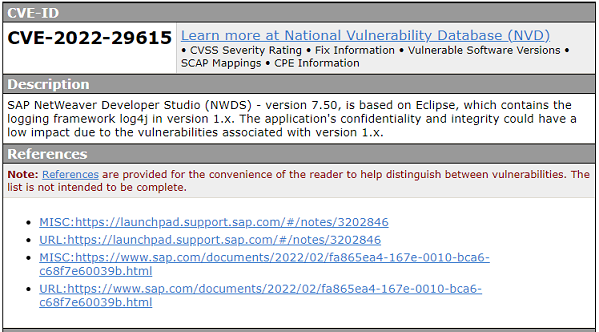
\includegraphics{cverecord}
	\caption[CVE Record]{CVE Record \source{\cite{CVEMITREWebsite}}}
	\label{fig:CVE Record}
\end{figure}

In order to make sure that all vulnerabilities listed in the \textit{CVE List} are unique and maintained properly, \textit{CVE IDs} can only be assigned and \textit{CVE Records} can only be published by MITRE and several partner organizations, so called \textit{CVE Numbering Authorities (CNA)}. Thus, to add a new vulnerability to the \textit{CVE List}, the discoverer has to report it to a CNA \cite{CVEWebsite}.\\

\noindent
\textbf{Common Vulnerability Scoring System (CVSS)}\\
\noindent
CVSS is an open framework for rating vulnerabilities. It is owned and managed by the non-profit organization \textit{Forum of Incident Response and Security Teams (FIRST)}. The framework captures the main characteristics of a vulnerability to produce a numerical score between 0.0 and 10.0 reflecting its severity.\par
Therefore CVSS is composed of three metric groups: Base, Temporal, and Environmental. The \textit{Base Score} considers the intrinsic characteristics of a vulnerability that are constant over time and assumes the worst case impact across different environments. These characteristics take into account exploitability metrics like attack complexity but also impact metrics like confidentiality impact. The \textit{Base Score} is typically calculated by the organization maintaining the vulnerable product or by third party analysts on their behalf. The \textit{Temporal Score} considers characteristics that may change over time but not across environments. Such a characteristic would be the maturity of exploit code. The \textit{Environmental Score} considers the relevance of a vulnerability in a specific environment. \textit{Temporal} and \textit{Environmental Scores} are typically calculated by the consumers of the components to adjust the vulnerability rating to their organizations use case and environment. These Scores can then be used for internal risk management \cite{CVSSSpec}.\\

\noindent
\textbf{Common Weakness Enumeration (CWE)}\\
\noindent
CWE is a community-developed list of software and hardware weaknesses maintained by MITRE. Each weakness in the least is assigned a\textit{ CWE ID}. The list represents weaknesses on different levels of abstraction. This is conceptually shown by figure \ref{fig:CWE Hierarchy}.

\begin{figure}[H]
	\centering
	
\includegraphics[scale=0.7]{cwehierarchy}
	\caption[CWE Hierarchy]{CWE Hierarchy \source{Own Representation}}
	\label{fig:CWE Hierarchy}
\end{figure}

\noindent
So there exist relationships between elements on different levels of abstraction. As shown \textit{Classes} are usually member of a \textit{Category} and might also be the child, hence a more concrete description, of a \textit{Pillar}. Additionally to what is shown in the figure, these relationships may also skip levels of hierarchy. Thus, a \textit{Base Level Weakness} may be a direct member of a \textit{Category} or a child of a \textit{Pillar}. An example for a Base Level Weakness is\textit{CWE}-478\textit{: Missing Default Case in Switch Statement} which is a member of \textit{Bad Coding Practices} and a child of the class \textit{Incomplete Comparison with Missing Factors}, which is a child of the pillar \textit{Incorrect Comparison} \cite{CWEWebsite}.\\

\noindent
\textbf{Common Platform Enumeration (CPE):} The CPE specification originally created by MITRE and now maintained by NIST provides a naming scheme for IT assets such as software. It may be used to uniquely determine a specific software and its version. This way a CPE enables cross referencing to other sources of information. The commonly used CPE naming scheme is structured as follows:\\
\noindent
\begin{lstlisting}[caption=CPE Formatted String Binding, captionpos=b, label=lst:CPE]
cpe:2.3: part : vendor : product : version : update : edition : language : sw_edition : target_sw : taget_hw : other
\end{lstlisting}

Thereby \lstinline|part| may be \textit{a} for applications, \textit{o} for operating systems, and \textit{h} for hardware devices. \lstinline|edition| is a legacy attribute in the current version of the specification and may be omitted where not required for backward compatibility. The attributes after \lstinline|edition| were newly introduced in this version and are referred to as \textit{extended attributes}. \lstinline|sw_edition| should characterize a particular market or class of users a product is tailored to (e.g. online), \lstinline|target_sw| a software computing environment (e.g. linux), \lstinline|target_hw| the instruction set architecture (e.g. x86), and \lstinline|language| the language supported in the user interface \cite{CPESpec}.\\

\noindent
\textbf{National Vulnerability Database (NVD)}\\
\noindent
The NVD is a database of vulnerabilities owned and maintained by NIST. In the paragraph about CVE, it was mentioned that the \textit{CVE Records} do not contain technical data, information about risks and impact, or fixes. The NVD feeds from the \textit{CVE List} and uses the information provided in the \textit{CVE Records} to perform further analysis. As a result, a NVD entry exists for each \textit{CVE ID} and provides a \textit{CVSS Base Score}, a \textit{CWE ID} and a \textit{CPE ID} \cite{NVDWebsite}.\par 
Thus, NVD combines all the aforementioned standards and concepts to provide thorough and concise human and machine-readable information about vulnerabilities. \textit{CPE IDs} identifying a particular software version in use may be queried against a NVD API to automatically check for known vulnerabilities. The \textit{CVSS Base Score} is a valuable foundation for internal risk assessment and the \textit{CWE ID} helps to quickly understand the type of a vulnerability.\\

\subsection{Software Bill of Materials}
A \textit{Software Bill of Materials} is an inventory of the components used in a software. It ideally contains all direct and transitive components and their dependencies, so it is in other words pretty much the dependency graph of a software \cite{OWASPWebsite,NTIASBOM}.\\

As consequence to an \textit{Executive Order on Improving the Nation's Cybersecurity}, the \textit{National Telecommunications and Information Administration (NTIA)} published a document describing the minimum requirements for SBOMs \cite{ExecutiveOrderSBOM,NTIASBOM}). According to this document, these are:

\begin{table}[H]
	\begin{tabularx}{\linewidth}{|l|X|}
		\hline
		\textbf{Data Fields (Metadata)} & Baseline information about each component: Supplier, Component Name, Version of the Component, Other Unique Identifiers, Dependency Relationship, Author of SBOM Data, Timestamp of SBOM creation \\
		\hline
		\textbf{Automation Support} & Automatic generation and machine-readability to allow for scaling across the software ecosystem. \\
		\hline
		\textbf{Practices and Processes} & Implementation of policies, contracts and arrangements to maintain SBOMs.\\
		\hline
	\end{tabularx}
	\caption[Minimum Elements of a SBOM]{Minimum Elements of a SBOM \source{\cite{NTIASBOM}}}
	\label{Tab:ElementsOfSBOM}
\end{table}

The goal of the \textit{Data fields} is to sufficiently identify the components to track them through the supply chain and map them to other data sources, such as vulnerability and license databases. The \textit{Automation Support} provides the ability to scale across the software ecosystem. The \textit{Practices and Processes} ensure the maintenance by integration into the ALM. SBOMs thereby increase software transparency, providing those who produce, purchase and operate software the means to perform proper risk assessments \cite{NTIASBOM}.\par
Due to this Executive Order, SBOMs are now required for all U.S. federal software procurements. This does not only affect direct software vendors of the U.S. government \cite{ExecutiveOrderSBOM}. As a consequence to this Executive Order, every organization that is downstream from the U.S. government in the supply chain may be required to provide SBOMs for its products. Thus, this will be a crucial capability for most software vendors.\par
There are three data formats mentioned in the minimum elements document which are interoperable, able to fulfill the requirements and either human- and machine-readable. Those are the \textit{Software Package Data eXchange (SPDX)}, \textit{CycloneDX} and \textit{Software Identification (SWID)} tags \cite{NTIASBOM}. SPDX is the most mature standard. It has laid out a lot of groundwork for the more recent CycloneDX. Thus, to get an better and more concrete understanding of SBOMs, SPDX will be examined in more detail.\\

\noindent   
\textbf{SPDX License List and License Identifiers}\\
SPDX is an initiative founded in 2010 and hosted at \textit{The Linux Foundation}. In 2021 the SPDX specification even became an ISO standard \cite{SPDXISO}. The initiative focuses on solving challenges regarding the licenses and copyrights associated with software packages. SPDX therefore assembles licenses and exceptions commonly found in OSS in the \textit{SPDX License List}. More precisely, this list includes a standardized short identifier, the full name, the license text, and a canonical permanent URL for each license and exception. By incorporating this \textit{SPDX License Identifiers} in source on file level, one enables automation of concise license detection, even if just parts of an OSS project are used. Furthermore, SPDX provides \textit{Matching Guidelines} to ensure that e.g. a \enquote{BSD 3-clause} license in a LICENSE file of an OSS project with different capitalization or usage of white space than the master license text included in the \textit{SPDX License List} is still identified as \enquote{BSD 3-clause} license.\\

\noindent
\textbf{SPDX Documents}
At the heart of the SPDX initiative are the \textit{SPDX Documents} which leverage the \textit{SPDX License List} and \textit{SPDX License Identifiers} to describe the licensing of a set of associated files, referred to as \textit{Package} in the context of SPDX. A \textit{SPDX Document} provides means to describe information about the document creation, the package as a whole, individual files, snippets of code within an individual file and other licenses that are not contained in the \textit{SPDX License List} but are still relevant for the package, relationships between \textit{SPDX Documents}, and annotations, which in a way are comments within an \textit{SPDX Document}. The concept of relationships is a rather new addition to the specification. It is particularly useful if one has an SPDX Document describing a binary. Explicitly capturing relationships like \enquote{generated from} these source files and \enquote{dynamically linking} these libraries allows for a complete licensing picture. \par
These documents may be represented in one of the following five file format: tag/value (.spdx), JSON (.spdx.json), YAML (.spdx.yaml), RDF/xml (.spdx.rdf), and spreadsheets (.xls) \cite{SPDXWebsite, SPDXSpec}.\\

\noindent
To give a more concrete idea of the basic concepts of \textit{SPDX Documents}, an example from the SPDX GitHub repository will be briefly examined \cite{SPDXExamples}. Therefore figure \ref{fig:C Project} below shows the directory structure of a \enquote{Hello World} project in C.

\begin{figure}[H]
	\centering
	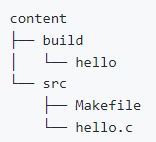
\includegraphics{directory_spdxexample}
	\caption[C Project Directory Structure]{C Project Directory Structure \source{\cite{SPDXExamples}}}
	\label{fig:C Project}
\end{figure}

\noindent
Listing \ref{lst:SPDX Document} shows a corresponding \textit{SPDX Document}. Some tag:value pairs which are less relevant for the overall understanding are deliberately omitted to contain the length of the example.\\ 

\noindent
\begin{lstlisting}[basicstyle=\tiny, caption=SPDX Document, captionpos=b, label=lst:SPDX Document]
SPDXVersion: SPDX-2.2
DataLicense: CC0-1.0
SPDXID: SPDXRef-DOCUMENT
DocumentName: hello
DocumentNamespace: https://swinslow.net/spdx-examples/example1/hello-v3
Creator: Person: Steve Winslow (steve@swinslow.net)
Created: 2021-08-26T01:46:00Z

##### Package: hello
PackageName: hello
SPDXID: SPDXRef-Package-hello
PackageDownloadLocation: git+https://github.com/swinslow/spdx-examples.git#example1/content
PackageLicenseConcluded: GPL-3.0-or-later
PackageLicenseInfoFromFiles: GPL-3.0-or-later
PackageLicenseDeclared: GPL-3.0-or-later
PackageCopyrightText: NOASSERTION

FileName: /build/hello
SPDXID: SPDXRef-hello-binary
FileType: BINARY
LicenseConcluded: GPL-3.0-or-later
LicenseInfoInFile: NOASSERTION
FileCopyrightText: NOASSERTION

FileName: /src/Makefile
SPDXID: SPDXRef-Makefile
FileType: SOURCE
LicenseConcluded: GPL-3.0-or-later
LicenseInfoInFile: GPL-3.0-or-later
FileCopyrightText: NOASSERTION

FileName: /src/hello.c
SPDXID: SPDXRef-hello-src
FileType: SOURCE
LicenseConcluded: GPL-3.0-or-later
LicenseInfoInFile: GPL-3.0-or-later
FileCopyrightText: Copyright Contributors to the spdx-examples project.

Relationship: SPDXRef-hello-binary GENERATED_FROM SPDXRef-hello-src
Relationship: SPDXRef-hello-binary GENERATED_FROM SPDXRef-Makefile
Relationship: SPDXRef-Makefile BUILD_TOOL_OF SPDXRef-Package-hello
\end{lstlisting}

\noindent
Most of the tag:value pairs are self-explanatory, but some might require some explanation. The \textit{Concluded License} is the license the SPDX file creator has concluded as the governing license of a package or a file. \textit{License Information from Files} contains a list of all licenses found in a package and the \textit{Declared License} is the license declared by the authors of the package \cite{SPDXSpec}. Additionally, listing \ref{lst:SPDX Document} illustrates how the concept of relationships may be used.\par
It is also worth mentioning that the concept of \textit{Packages} in SPDX as a set of associated files is really rather loose. Thus, describing the project in figure \ref{fig:C Project} as two separate packages, one for source and one for binary, optionally in the same or also in two separate \textit{SPDX Documents} would be completely conform with the specification as well.\par
Since SPDX has been around for so long and is an accepted ISO standard, there exists a lot of useful tooling. It is therefore quite easy to automate tasks like producing, consuming, transforming and validating \textit{SPDX Documents} \cite{SPDXWebsite}.\\
 
\subsection{Regulations}
Vulnerabilities and licenses are not the only risks associated with enterprise software. Companies also need to consider governmental regulations since violations may lead to fines that have critical impact on the business.\\

\noindent
\textbf{Export Control Classification Number (ECCN)}\\
\noindent
The ECCN is a 5 character alpha-numeric designation used to determine whether an so called dual-use item needs an export license from the U.S. Department of Commerce in order to legally export it. Dual-use items are items that may be used for civil as well as military purposes. The ECCN gives some information about the product, as shown in figure \ref{fig:ECCN Structure} below.

\begin{figure}[H]
	\centering
	
\includegraphics[scale=0.6]{eccn}
	\caption[ECCN Structure]{ECCN Structure \source{\cite{ECCN}}}
	\label{fig:ECCN Structure}
\end{figure}

All ECCNs are listed in the \textit{Commerce Control List (CCL)}. The entries in the list contain information about why an item might be under export control regulations. In the top of figure \ref{fig:ECCN Structure} is a snippet of such an entry. The reason for the export regulations of products with the classification number 4E993 is AT, which is the abbreviation for Anti-Terrorism \cite{ECCN}.\par


\todo{A lot of these standards could be explained in much more detail (at the moment, they are kept just as long as currently deemed necessary to understand the further topics).}

\section{Context at SAP Gardener}
Builds, Repositories, Gardener Servicelet Pattern (Session mit Uwe)
\subsection{SAP Gardener}
\subsection{SAP Gardener Deployment Scenario}
\subsection{Open Component Model}
\section{Integration into the Application Lifecycle}